\chapter{近简并能带电子的磁性质}

在磁场中布洛赫电子的准经典理论中,量子化条件不仅仅是朗道能级的简洁描述,而且是输运性质\cite{SdH}和热力学性质\cite{dHvA}的量子振荡的定量理论的基石。 Onsager\cite{Onsager}和Lifshitz\cite{lifshitz_kosevich,lifshitz_kosevich_jetp}给出的最初的量子化条件忽略了自旋轨道耦合。随后Roth\cite{rotheffham,rothmag},Mikitik\cite{Mikitik_quantizationrule}以及本文作者及合作者\cite{topoferm,100p}将自旋轨道耦合效应考虑了进来,但是得到的量子化条件仅仅适用于自旋轨道耦合效应远远大于(或者远远小于)塞曼作用能。


到目前为止,我们还没有看到一个能够将自旋轨道耦合和塞曼劈裂同等处理的量子化条件。对于没有空间反演的具有自旋轨道耦合的材料,或者是具有磁序的材料,这样的一个量子化条件非常重要。这些材料具有一个自旋二分之一的自由度,并且能带的自旋简并被自旋轨道耦合或者磁序微弱地劈开。一个典型的例子就是具有Rashba自旋轨道耦合的二维电子气:
\begin{equation}
H_R=\frac{{\hbar^2} k^2}{2m}+\hbar\alpha  (k_{x}\sigma_{y}-k_{y}\sigma_{x}).\label{eq:Rashba-Hamiltonian}
\end{equation}
考虑加上一个$-z$方向的磁场,我们主要关注能量远大于$m\alpha^2$的地方。这里,磁振子轨道【见图\fig{fig:orbits}(a)】在$\bk$空间被自旋轨道耦合劈开,其面积之差为$\delta S$,其中$\delta S$远小于两个轨道的面积的平均值$S$\footnote{式\ref{deltaSvsS}中 $\delta S$ 和 $S$ 的表达式在$E{\gg}m\alpha^2$时渐进正确。}:
\e{\delta S = 4\pi m \alpha k_E/\hbar\ll S =\pi k_E^2; \;\; k_{E}:=\f{\sqrt{2m E}}{\hbar}.\label{deltaSvsS}}
$S$ 也是在没有自旋轨道耦合的时候的磁振子的面积($\alpha{=}0$)。

\begin{figure}
	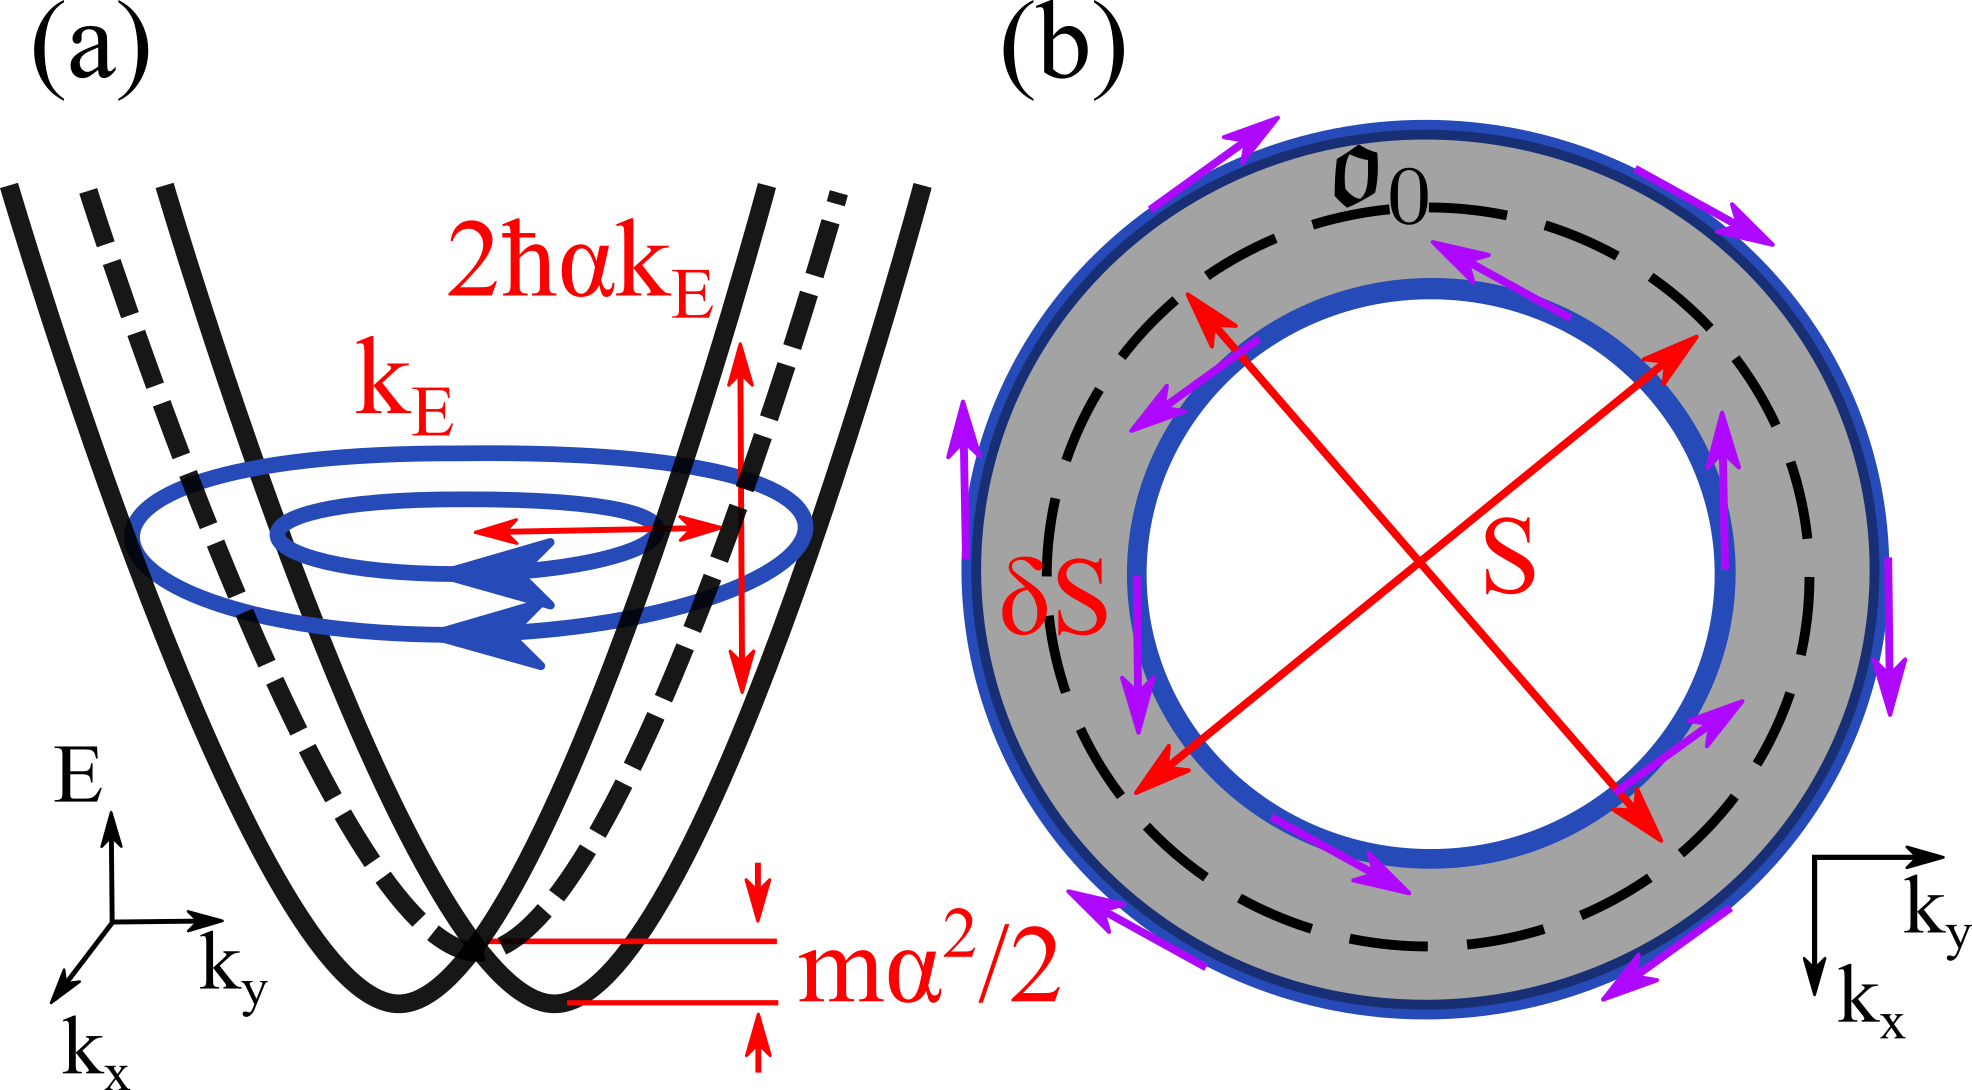
\includegraphics[width=0.8\textwidth]{../figures/orbits.png}
	\centering
	\caption{(a) 实线(虚线)阐释了具有(没有)Rashba自旋轨道耦合的二位电子气的能带色散。图中具有方向的圆代表了磁振子轨道,其中磁场方向为$-z$方向。 (b) 虚的圈$S$标注出了零阶轨道$\frako_0$;$\delta S$是自旋轨道耦合劈裂的轨道的面积之差;紫色的箭头标出了自旋结构。\label{fig:orbits}}
\end{figure}

我们的工作给出了一个适用于近简并能带的推广的量子化条件,这个量子化条件的适用范围包括具有自旋轨道劈裂的能带。我们定义近简并为磁振子面积的差远小于磁振子面积的平均值$|\delta S/S|{\ll}1$。我们提出的量子化条件还依赖于另一个条件:$S$远大于$1/l^2$,这里的$l$事磁长度$l{=}\sqrt{\hbar/eB}$;这个条件也是标准的准经典Onsager-Lifshitz-Roth理论假设。通过引入两个小量$|\delta S/S|$和$1/l^2|S|$,我们的研究推广深化了前人仅仅基于一个小量的准经典理论\cite{kohn_effham,blount_effham,rotheffham,wannier_fredkin,fischbeck_review,Mikitik_quantizationrule,topoferm,100p,gao_zero-field_2017}。

$1/l^2|\delta S|$量化了由塞曼能导致的近简并的轨道的耦合。在$l^2|\delta S|{\gg}1$的情况下,Onsager-Lifshitz{-Roth}量子化条件可以分别作用在两个共心但是不耦合的磁振子轨道。在另外一个极限$l^2|\delta S|{\ll}1$,自旋轨道耦合导致的劈裂可以忽略,我们可以采用已有的严格简并能带的量子化条件\cite{rotheffham,rothmag,topoferm,100p,Mikitik_quantizationrule}。我们的统一的量子化条件给出了介于前述的两个极限情况下的朗道能级的解($l^2|\delta S|{\sim}1$),这种情况下,塞曼能和自旋轨道耦合的能量基本相同;而前人的工作仅仅展示了这两个能量一个远大于另一个的情况下的量子化条件。我们工作给出了在任意对称群的具有自旋轨道耦合的晶体的量子化条件。章节\ref{sec:qtznrules}描述了这个近简并能带的量子化条件,其中哦我们假设了一个自旋二分之一(或者赝自旋二分之一)的自由度。正如章节\ref{sec:discussion}所述,我们的量子化条件能够涵盖任意带数的近简并能带的朗道量子化。


在章节\ref{sec:Rashba}中,我们利用具有Rashba和Dresselhaus自旋轨道耦合的二维电子气,证明了我们的量子化能级的有效性。如果给具有Rashba自旋轨道耦合的二维电子气加上足够强的面内磁场,能带中的Dirac点不仅仅会移动,而且会倾斜,成为一个第二类的狄拉克点\cite{soluyanov_type-ii_2015, muechler_tilted_2016, bergholtz_topology_2015}。在章节\ref{sec:inplanezeeman}中,我们研究了第二类狄拉克点附近的Landau-Zener隧穿现象。特别的,我们将要证明我们的量子化条件囊括了近简并能带之间的量子隧穿,这个现象被称为带间的磁隧穿\cite{kaganov_coherent_1983,slutskin_dynamics_1968,AALG,100p}。我们将要认真研究一个最近提出的二类狄拉克点附近的完美Klein隧穿的现象\cite{obrien_magnetic_2016},我们发现如果考虑了塞曼效应的话,这个完美隧穿永远不会发生。


\section{量子化条件{sec:qtznrules}}

首先让我们大致解释一下这个量子化条件是怎么出现的;我们将这个量子化条件的分步的严格的证明留到附录\ref{app:quantizationruleproof}中。我们要考虑的是一个没有加磁场的时候有着离散平移不变性的哈密顿量: $\hat{H}_0{+}\delta \hat{H}$。前面的这个分解要求$\hat{H}_0$的能带在每一个波矢$\bk$处是$D$重简并的,而$\delta \hat{H}$则作为微扰破除这个$D$重简并。简单起见,我们假设$D{=}2$的自旋简并,$D>2$的情形则留在附录\ref{app:quantizationruleproof}中讨论。一个简单的例子是$\hat{H}_0$是薛定谔哈密顿量,而$\delta \hat{H}$是自旋轨道耦合的哈密顿量;另一个例子是$\hat{H}_0$是具有空间反演的包含自旋轨道耦合的泡利哈密顿量,而$\delta \hat{H}$是一个晶格畸变,轻微破坏了空间反演对称性。

现在让我们加上一个磁场,我们首先考虑忽略$\delta \hat{H}$和塞曼效应的自旋简并的朗道能级。在准经典的描述下,我们对$\hat{H}_0$的低能简并的能带的磁场动力学性质进行考察,这条能带的色散记为$\var(\bk)$。比如说,对于Rashba模型,$\var(\bk){=}\hbar^2 k^2/2m{+}\order(k^4)$。众所周知,朗道量子化是由Peierls修正得到的$\var(\bk){\rightarrow}\var(\bK)$\cite{peierls_substitution},这里的$\boldsymbol{K}{:}{=}\boldsymbol{k}{+}(e/\hbar) \boldsymbol{A}(i\nabla_{\boldsymbol{k}})$,并且$\boldsymbol{A}(\br)$是矢势。我们假设磁场沿着$-z$方向,$[K_x,K_y]{=}i\lmt$。准经典的波函数的解对应着电子在$\var(\bk)$的等能面作回旋运动【见图\ref{fig:orbits}(b)】,这个蕴含着电子运动方向(运动方程为$ \hbar dk_{\alpha}/dt {=} \lmt \epsilon_{\ab}\partial \var/\partial k_{\beta} $,其中 $\epsilon_{xy}{=}{-}\epsilon_{yx}{=}1$)的轨道被称为零阶轨道$\frako_0$。在这个工作中,我们仅仅关注闭合的轨道,闭合的意思指的是轨道不会横穿布里渊区。

朗道能级的量子化条件反映了WKB准经典波函数在轨道$\frako_0$上的单值性\cite{berry_mount_review},换句话说,电子在一个磁振子周期$T_c$中获得的相位是$2\pi$的整数倍:$(l^2S(E){+}\gamma)/2\pi{\in}\Z$。最高阶的相位是是$l^2S{:}{=}{-}l^2\int_{0}^{T_c} k_x \dot{k}_y dt$;$S$同时也可以阐释为具有正负号(对于电子型的轨道是正的)的$\bk$空间$\frako_0$的面积,见图\ref{fig:orbits}(b)。$\gamma$是第二阶的Maslov相位修正\cite{keller1958},这个修正等于$\frako_0$绕的圈数$r$乘以$\pi$,也就是切向量的绕圈数)\cite{100p};对于一个能够连续变化为圆的轨道,$r{=}{\pm} 1$。在零阶近似下,所有的朗道能级是自旋简并的,能级间隔是
\e{ \var_c:=\f{2\pi}{l^2|\partial S/\partial E|}:=\f{\hbar^2}{ml^2}:=\f{h}{T_c}. \label{def:cyclotron}}
这里,$\var_c$和$T_c$分别是零阶轨道的磁振子能量和周期,$m$是有效质量。下面开始,朗道能级的简并指的就是自旋简并。


